\documentclass[a4paper,12pt]{report}
\usepackage[utf8]{inputenc} % Codificação de caracteres UTF-8
\usepackage[brazil]{babel} % Idioma Português do Brasil
\usepackage{geometry} % Pacote para ajuste das margens
\usepackage{graphicx} % Inclusão de imagens
\usepackage{lipsum} % Texto de preenchimento
\usepackage{setspace} % Espaçamento
\usepackage{titling} % Pacote para título e subtítulo
\usepackage{longtable}
\usepackage{enumitem}
% Definir margens do documento
\geometry{left=3cm, right=2cm, top=3cm, bottom=2cm}
\usepackage[utf8]{inputenc} % Codificação de caracteres
\usepackage[brazil]{babel} % Idioma
\usepackage{graphicx} % Pacote para inclusão de imagens
\usepackage{geometry} % Pacote para ajustar margens
\usepackage{hyperref} % Pacote para links clicáveis
\usepackage{titlesec} % Personalizar títulos
\usepackage{lipsum} % Pacote para texto de preenchimento
\usepackage{hyperref}


% Estilo para os títulos de capítulo
\titleformat{\chapter}[hang]
  {\normalfont\huge\bfseries}{\thechapter.}{20pt}{\huge}

% Definir capa - formatar melhor 
\title{\textbf{Plataforma de Agendamento Online para Consultas Psicológicas}\vspace{70mm}}
\author{
  Vinicius Gustierrez Neves - 14749363 \\
  Catarina Moreira Lima - 8957221 \\
  Pietra Gullo Salgado Chaves - 14603822 \\
  Christian Bernard S. C. G. Ribeiro - 11795572
}
\begin{document}

% Capa
\maketitle
\newpage

% Sumário
\tableofcontents
\newpage

% 1. Seção: Introdução
\chapter{Introdução}

\section{Objetivo do Sistema}
Atualmente, o processo de agendamento de atendimentos psicológicos oferecidos pela USP São Carlos, por meio de programas como o \href{https://www.puspsc.usp.br/saude-mental/}{Apoia USP}, é marcado por uma experiência pouco prática e burocrática. Agendamentos são feitos por e-mail, telefone ou preenchimento de formulários, dificultando a personalização do atendimento. Além disso, modificar consultas ou verificar horários disponíveis é um processo complicado, sem uma interface centralizada. A dependência de intervenção humana gera atrasos e gargalos, especialmente diante do alto volume de solicitações, e as informações sobre os programas de apoio psicológico são de difícil acesso, tornando o processo ainda mais desafiador para a comunidade.\\

O sistema proposto visa otimizar a gestão e o agendamento de consultas psicológicas para a comunidade do Campus USP São Carlos, oferecendo uma plataforma que agiliza e simplifica o processo tanto para pacientes quanto para profissionais.\\

Para os pacientes, o novo sistema proporcionará uma experiência mais simples e eficiente, permitindo o agendamento rápido e personalizado de consultas sem a necessidade de processos manuais. A plataforma permitirá visualizar, alterar ou cancelar consultas de forma automática e intuitiva, sem burocracias.\\

Para os profissionais, a solução oferecerá um sistema integrado de gestão de agendas, facilitando a organização e atualização dos horários de atendimento. A automatização de remarcações e cancelamentos reduzirá significativamente o tempo gasto com tarefas administrativas, permitindo que os psicólogos se concentrem mais no atendimento clínico. Além disso, o acesso a informações sobre os programas de apoio psicológico será mais acessível, promovendo um fluxo de atendimento mais ágil e menos burocrático para a comunidade acadêmica.\\

\section{Atores e Stakeholders}
% Descrição dos diversos atores e stakeholders.
\begin{itemize}
    
    \item \textbf{Profissionais da Plataforma (Ator e Stakeholder):}
    São os psicólogos responsáveis por cadastrar suas informações, disponibilizar horários para atendimento e definir a dinâmica das consultas. Eles podem visualizar e editar os agendamentos realizados, acessar informações dos pacientes e consultar relatórios de consultas.\\
    
    \textbf{Por que utilizariam a plataforma?}
    \begin{itemize}
        \item \textbf{Gerenciamento Simplificado:} Organização prática da agenda, com remarcações e cancelamentos automatizados, sem necessidade de comunicação direta com pacientes.
        \item \textbf{Visualização Centralizada:} Todos os agendamentos e informações dos pacientes em um único lugar.
        \item \textbf{Redução de No-Shows:} Lembretes automáticos que ajudam a evitar faltas.\\
    \end{itemize}
    
    \item \textbf{Usuários Pacientes (Ator e Stakeholder):}
    São alunos da USP que utilizam a plataforma para agendar consultas psicológicas de forma rápida e personalizada, escolhendo profissionais conforme suas preferências e necessidades. O sistema permite o cadastro de informações pessoais e a visualização de psicólogos e horários disponíveis, além de facilitar o cancelamento e remarcação de consultas.\\
    
    \textbf{Por que utilizariam a plataforma?}
    \begin{itemize}
        \item \textbf{Facilidade no Agendamento:} Agendamento rápido e simples, adaptado ao cotidiano dos estudantes.
        \item \textbf{Acesso a Diversos Profissionais:} Opções de psicólogos com diferentes especializações e abordagens terapêuticas.
        \item \textbf{Acessibilidade e Flexibilidade:} Consultas podem ser agendadas ou alteradas a qualquer momento.\\
    \end{itemize}

    \item \textbf{Administrador do Sistema (Ator e Stakeholder):}
    Responsável pela manutenção geral da plataforma, incluindo gerenciamento de usuários e profissionais, cadastro de horários, implementação de melhorias e leitura de feedbacks e relatórios.\\

    \textbf{Por que utilizariam a plataforma?}\\
    Para garantir a operação eficiente e organizada da plataforma, otimizando a experiência dos usuários e o desempenho do sistema.\\

    \item \textbf{Universidade (Stakeholder):}
    A USP apoia o projeto ao fornecer infraestrutura e suporte técnico, visando melhorar o bem-estar da comunidade acadêmica com serviços psicológicos eficientes e organizados. O sistema também reflete positivamente na responsabilidade social e acadêmica da instituição.

    \item \textbf{Comunidade do Campus USP São Carlos (Stakeholder):}
    Alunos, professores e funcionários se beneficiam diretamente do sistema, que facilita o acesso aos serviços psicológicos, promovendo organização e acessibilidade no atendimento. Isso contribui para o bem-estar geral da comunidade e engaja os usuários no cuidado da saúde mental.
    
\end{itemize}


\section{Principais Funcionalidades}
% Descrição das principais funcionalidades pretendidas.
As principais funcionalidades do sistema incluem:

\begin{itemize}
    \item \textbf{Cadastrar informações pessoais:} Permite que tanto os pacientes quanto os psicólogos realizem seu cadastro na plataforma, inserindo suas informações pessoais e profissionais de forma segura.

    \item \textbf{Sistema de Login:} Permite que os diferentes usuários da plataforma, tanto pacientes quanto psicólogos, acessem suas contas de forma segura utilizando seus e-mails e senhas. Para os alunos, o login deve ser realizado com o e-mail institucional da USP, enquanto os profissionais podem utilizar qualquer e-mail de sua escolha, sem restrições.
    
    \item \textbf{Agendamento de consultas:} Pacientes podem visualizar os psicólogos disponíveis, bem como suas informações, e escolher horários livres para agendar consultas de forma rápida e fácil.

    \item \textbf{Cancelar/remarcar agendamentos:} Os pacientes podem cancelar ou remarcar suas consultas diretamente na plataforma, com os horários disponíveis sendo automaticamente atualizados. Um e-mail é enviado ao outro usuário, avisando a modificação na agenda.
    
    \item \textbf{Conferir agendamentos feitos:} Os psicólogos e pacientes podem visualizar todos os agendamentos realizados, organizados por data e horário, permitindo um controle eficiente da agenda de atendimentos. 
    
    \item \textbf{Gerenciar perfis de usuários:} Administradores podem acessar os perfis dos usuários (pacientes e psicólogos), visualizar suas consultas marcadas, e acompanhar o histórico de atendimentos, garantindo que as informações estejam sempre atualizadas e consistentes.

    \item \textbf{Visualizar perfis de usuários:} Psicólogos podem acessar algumas informações cadastradas pelos usuários, de forma a permitir uma compreensão inicial de seus pacientes.
    
    \item \textbf{Obter relatórios e feedbacks:} Administradores do sistema possuem a capacidade de gerar relatórios detalhados sobre o uso da plataforma. Esses relatórios incluem informações como o número de usuários cadastrados e ativos, quantidade de psicólogos registrados, volume de consultas realizadas, além de identificar horários mais demandados. Paralelamente, tanto psicólogos quanto pacientes podem fornecer feedbacks
    sobre o sistema, seja reportando bugs, sugerindo melhorias ou comentando sobre a
    experiência de uso da plataforma

    \item \textbf{Contatar pacientes:} O psicólogo tem a possibilidade de entrar em contato com o paciente diretamente por meio de mensagens. Esse contato pode abranger temas como confirmações ou mudanças em consultas agendadas, novos horários de atendimento, cancelamentos, ou outros tópicos relevantes ao tratamento. 
    

\end{itemize}


\section{Resultados Obtidos} Ao longo da disciplina, foram realizados diversos exercícios semanais, que abordaram diferentes aspectos do sistema proposto, proporcionando uma visão abrangente e progressiva do projeto. A seguir, serão descritas as principais modelagens desenvolvidas, detalhadas nos capítulos subsequentes:

\begin{itemize} 
\item \textbf{Capítulo 2 - Especificação de Requisitos:} Desenvolvimento de histórias de usuário, definição de personas, criação do diagrama de casos de uso, e especificação textual e abstrata dos casos de uso. 
\item \textbf{Capítulo 3 - Arquitetura do Sistema:} Elaboração de um diagrama de arquitetura, acompanhado da descrição dos principais componentes e suas respectivas responsabilidades. 
\item \textbf{Capítulo 4 - Diagrama de Classes:} Definição das classes, atributos, visibilidade dos atributos, além dos relacionamentos e multiplicidade entre as classes. 
\end{itemize}

\chapter{Especificação de Requisitos}

Nesta seção, são detalhadas as etapas de levantamento e modelagem dos requisitos do sistema, essenciais para garantir que o desenvolvimento atenda às necessidades dos usuários e stakeholders. Os requisitos foram organizados de forma progressiva, desde histórias de usuário e personas, passando pelo diagrama de casos de uso, até a especificação textual dos casos de uso, tanto em formato abstrato quanto estendido. 
\\

%{Perfis de Usuários} - tem que ver o que vai fazer
%onde isso vai etc
Inicialmente, foram levantadas as principais classes de perfis de usuário para o sistema sistema de agendamento online de consultas, considerando uma aplicação para atendimentos com profissionais psicólogos. \\
\\
Para tal, os seguintes perfis descrevem as diferentes características e necessidades dos usuários deste sistema:
\begin{itemize}
    \item \textbf{Administrador do sistema:} 
É a pessoa responsável pela manutenção geral do sistema, como o gerenciamento dos perfis de usuários e profissionais da plataforma, cadastro dos horários disponíveis para atendimento, implementação de mudanças e leitura de feedbacks e relatórios da plataforma.

\item \textbf{Profissionais da plataforma:}

Serão os profissionais psicólogos responsáveis pelo cadastramento de suas informações pessoais, dos horários disponíveis para os seus agendamentos e do funcionamento/dinâmica de seus atendimentos. Eles poderão conferir os agendamentos realizados pelos seus usuários, bem como as informações pessoais dos dos seus pacientes.

\item \textbf{Usuários pacientes:}

Indivíduos pertencentes à comunidade da USP de São Carlos que desejem utilizar a plataforma a fim de agendar consultas com um profissional psicólogo dentre as opções existentes. Eles poderão cadastrar suas informações pessoais, a fim de facilitar um prévio conhecimento por parte dos profissionais, visualizar os profissionais disponíveis, bem como suas informações pessoais e seus horários de atendimento, e agendar novos ou cancelar/remarcar seus agendamentos.

\end{itemize}

\section{Histórias de Usuário}
Cada história de usuário representa as necessidades dos diferentes perfis de usuários do sistema em exemplos fictícios. Algumas das histórias de usuário produzida nos exercícios da disciplina foram:

\subsection{História de Usuário 1 - Ana (Paciente)}
\begin{itemize}
    \item Como paciente, Ana gostaria de saber os horários disponíveis para atendimento psicológico.
    \item Como paciente, Ana gostaria de saber mais sobre o/a profissional que realizará o atendimento e buscar o que melhor a atenda.
    \item Como paciente, Ana gostaria de poder marcar / desmarcar consultas pelo site.
    \item Como paciente, Ana gostaria de cadastrar seu perfil e informações pessoais para que possa ser contatada sobre as consultas.
    \item Como paciente, Ana gostaria de escolher um profissional dentre os disponíveis, com o objetivo de encontrar o que melhor se adequa a suas preferências.
\end{itemize}

\subsection{História de Usuário 2 - Carlos (Administrador do Sistema)}
\begin{itemize}
    \item Como administrador do sistema, Carlos gostaria de gerenciar os perfis dos usuários, para garantir que apenas pessoas autorizadas tenham acesso à plataforma.
    \item Como administrador do sistema, Carlos gostaria de cadastrar e atualizar os horários disponíveis para os atendimentos, garantindo que a plataforma esteja sempre atualizada.
    \item Como administrador do sistema, Carlos gostaria de implementar mudanças no sistema de acordo com o feedback dos usuários, para melhorar a experiência de uso da plataforma.
    \item Como administrador do sistema, Carlos gostaria de acessar e analisar relatórios de uso da plataforma, para identificar áreas que precisam de melhorias.
    \item Como administrador do sistema, Carlos gostaria de ser notificado sobre problemas técnicos ou de segurança, para poder agir rapidamente na resolução.
\end{itemize}

\subsection{História de Usuário 3 - Juliana (Psicóloga)}
\begin{itemize}
    \item Como profissional psicóloga, Juliana gostaria de cadastrar seus horários de atendimento, para que os pacientes possam agendar suas consultas com base em sua disponibilidade.
    \item Como profissional psicóloga, Juliana gostaria de acessar as informações dos pacientes agendados, para se preparar adequadamente para cada consulta.
    \item Como profissional psicóloga, Juliana gostaria de atualizar suas informações pessoais e profissionais no sistema, para que os pacientes possam conhecer seu perfil e abordagem terapêutica.
    \item Como profissional psicóloga, Juliana gostaria de ser notificada sobre novos agendamentos e cancelamentos, para organizar sua agenda de maneira eficiente.
    \item Como profissional e mãe de dois filhos, Juliana gostaria de poder contatar e reagendar ou cancelar com consultas marcadas com seus pacientes quando houver imprevistos em sua rotina.
    \item Como profissional psicóloga, Juliana gostaria de poder visualizar de maneira fácil suas consultas da semana.
    \item Como profissional psicóloga, Juliana gostaria de poder agendar consultas para seus pacientes recorrentes para acelerar esse processo.
\end{itemize}

\subsection{História de Usuário 4 - Natália (Paciente)}
\begin{itemize}
    \item Como estudante de Engenharia Elétrica, Natália gostaria de poder agendar horários de atendimento psicológico em momentos em que está livre, para que ela possa conciliar as consultas com sua agenda cheia.
    \item Como estudante metódica, Natália gostaria de poder escolher uma profissional psicóloga que tenha uma abordagem analítica, para que ela possa receber um suporte mais focado em técnicas e análises durante as sessões, especialmente em momentos de autocobrança.
    \item Como uma pessoa que valoriza a privacidade, Natália gostaria de poder compartilhar suas informações pessoais com os psicólogos de forma segura e controlada, para que apenas os profissionais envolvidos diretamente no seu atendimento possam acessar seus dados.
    \item Em semanas de avaliações, Natália gostaria de poder remarcar ou até cancelar suas consultas com antecedência, de forma a poder organizar a sua agenda e evitar a ausência em consultas que poderiam ser utilizadas por outros alunos do Campus.
    \item Natália costuma checar seus e-mails diariamente e gostaria de ser avisada, de preferência, por meio deles, quando houver algum imprevisto com o/a profissional que a atenderia.
\end{itemize}

\section{PERSONAS}
As personas representam perfis fictícios, porém realistas, que refletem os principais tipos de usuários que irão interagir com o sistema. Essas personas foram criadas para capturar as características, necessidades e expectativas de cada grupo de usuários, facilitando o entendimento das funcionalidades e aprimorando o design e a experiência de uso do sistema.


O uso dessas personas permite que a equipe de desenvolvimento considere as necessidades específicas de cada tipo de usuário ao projetar e implementar as funcionalidades do sistema, resultando em uma plataforma mais eficaz e adequada para todos os envolvidos.


A seguir, são apresentadas as três principais personas do sistema: o administrador, o paciente e o profissional psicólogo.


% Persona 1 - Administrador
\subsection{Persona 1: Administrador do Sistema}
\begin{minipage}{0.3\textwidth}
    \centering
    
\includegraphics[width=1.0\textwidth]{fotor-ai-20240915202734.jpg}
\end{minipage}
\hfill
\begin{minipage}{0.65\textwidth}
    \textbf{Nome:} Carlos Souza \\
    \textbf{Idade:} 33 anos \\
    \textbf{Profissão:} Administrador de Sistemas \\
    \textbf{Descrição:} Descrição: Carlos é formado em Ciência da Computação na USP e trabalha como administrador de sistemas há 10 anos. Ele é meticuloso e gosta de manter tudo em ordem. No trabalho, Carlos é responsável por gerenciar diferentes plataformas e sistemas, incluindo a plataforma de agendamentos de consultas para os estudantes da USP de São Carlos. Ele valoriza a eficiência e a funcionalidade no seu dia a dia e acredita que um sistema bem administrado contribui para uma experiência positiva dos usuários.\\
    \textbf{Casos de Uso:} UC11, UC12, UC13.
\end{minipage}

\vspace{1cm} % espaçamento entre as personas

% Persona 2 - Paciente
\subsection{Persona 2: Paciente}
\begin{minipage}{0.3\textwidth}
    \centering
    
\includegraphics[width=1.0\textwidth]{Screenshot from 2024-10-16 15-05-46.png}
\end{minipage}
\hfill
\begin{minipage}{0.65\textwidth}
    \textbf{Nome:} Ana Maria \\
    \textbf{Idade:} 19 anos \\
    \textbf{Profissão:} Estudante \\
    \textbf{Descrição:} Ana tem 19 anos e é uma estudante do curso de Matemática no ICMC. Ela possui uma irmã mais velha e um irmão mais novo, e se mudou de uma cidade em outro estado para ingressar na faculdade. Ana participa de atividades extracurriculares, as quais realizam reuniões pela tarde regularmente. Seu curso tem aulas majoritariamente noturnas. Já em seu segundo ano de graduação, Ana se vê mais cansada do que o comum, e se interessou pelo serviço de apoio psicológico fornecido pela USP.\\
    \textbf{Casos de Uso:} UC01, UC02, UC03, UC04, UC05, UC06, UC10.
\end{minipage}

\vspace{1cm} % espaçamento entre as personas

% Persona 3 - Psicólogo
\subsection{Persona 3: Profissional Psicólogo}
\begin{minipage}{0.3\textwidth}
    \centering
    
\includegraphics[width=1.0\textwidth]{fotor-ai-20240915203048.jpg}
\end{minipage}
\hfill
\begin{minipage}{0.65\textwidth}
    \textbf{Nome:} Juliana Ferreira \\
    \textbf{Idade:} 29 anos \\
    \textbf{Profissão:} Psicóloga \\
    \textbf{Descrição:} Juliana é psicóloga formada na FFCL-RP e possui experiência em atendimento clínico e comunitário para estudantes de diferentes faixas etárias. Ela trabalha com uma abordagem centrada na pessoa e acredita na importância de um atendimento humanizado e personalizado. Juliana valoriza a organização e a flexibilidade em seu trabalho, por isso procura manter sua agenda sempre atualizada para acomodar seus pacientes da melhor forma possível. Além do trabalho, ela gosta de ler, praticar yoga e se atualizar sobre novas técnicas e abordagens terapêuticas.\\
    \textbf{Casos de Uso:} UC01, UC02, UC03, UC04, UC05, UC06, UC07, UC08, UC09.
\end{minipage}

\section{Diagrama de Casos de Uso}

O Diagrama de Casos de Uso é uma ferramenta fundamental no processo de modelagem de sistemas, especialmente em sistemas orientados a objetos. Ele tem como objetivo representar de maneira visual como os diferentes tipos de usuários (atores) interagem com o sistema, destacando as principais funcionalidades que o sistema oferece. No contexto do sistema de atendimento de psicólogos, este diagrama mapeia as interações dos três principais tipos de atores — Psicólogo, Paciente e Administrador — com as funcionalidades disponíveis no sistema.

\begin{figure}[h!]
    \centering
    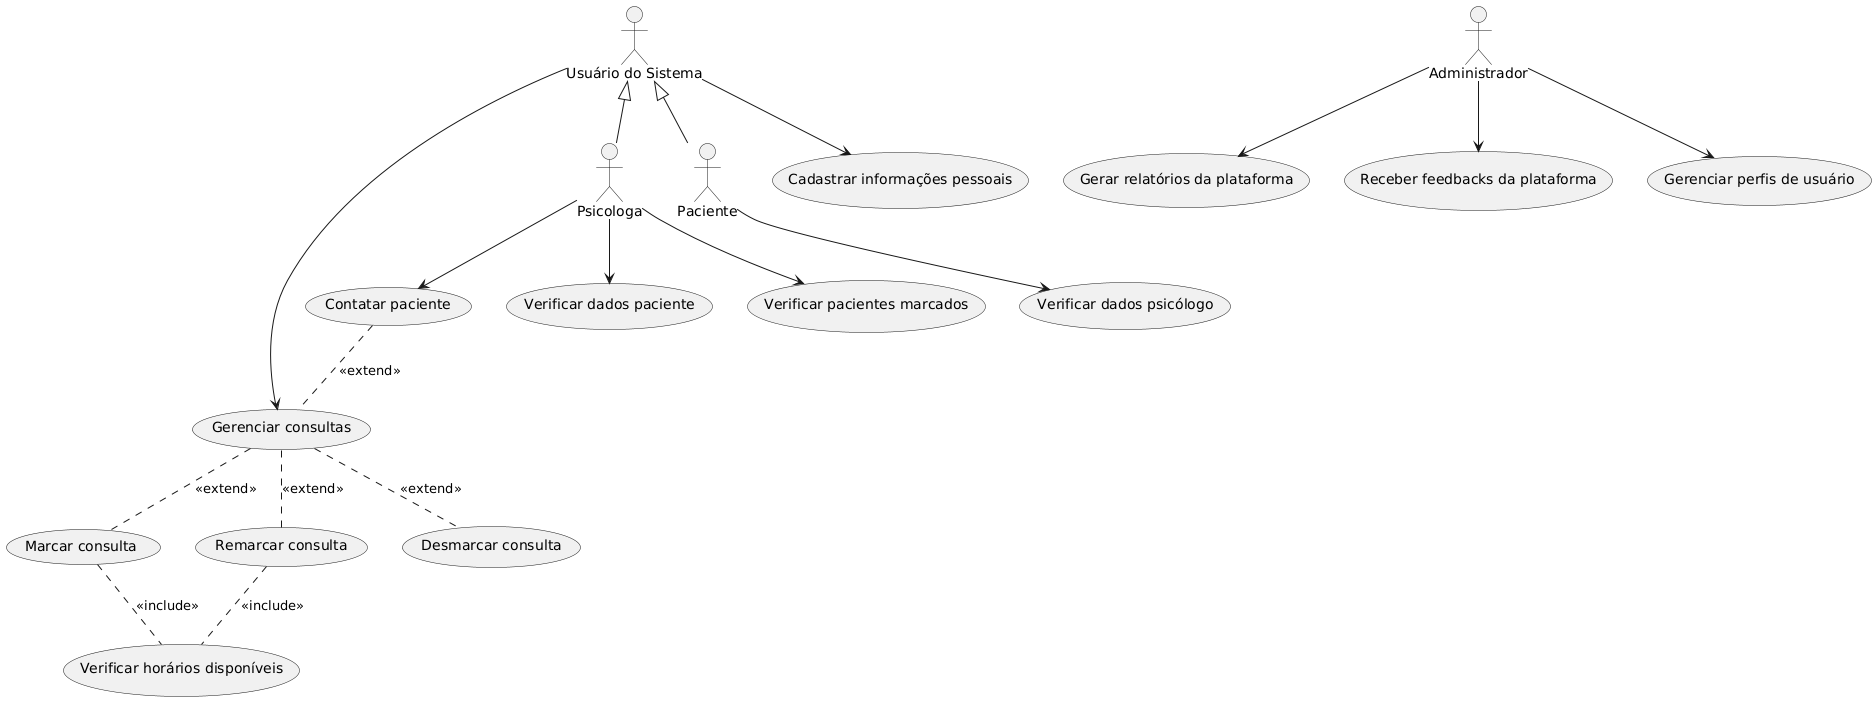
\includegraphics[width=1.0\textwidth]{casos de uso.png} % Substitua pelo nome do seu arquivo de imagem
    \caption{Diagrama de Casos de Uso em sua representação visual}
    \label{fig:exemplo}
\end{figure}

\section{Tabela com IDs de Casos de Uso}

% {Marcar Consulta:} Permite o agendamento de uma consulta em horários disponíveis, tanto para o paciente quanto para o psicólogo. 
% {Gerenciar Consultas}
% {Cadastrar Informações Pessoais}
% {Remarcar Consulta:} Permite reagendar uma consulta em horários disponíveis, tanto por iniciativa do paciente quanto do psicólogo.
% {Desmarcar Consulta:} Permite o cancelamento de consultas por parte do paciente ou do psicólogo.
% {Verificar Horários Disponíveis:} Facilita a visualização dos horários disponíveis para agendamento ou remarcação de consultas.
% {Contatar Paciente}
% {Verificar Dados do Paciente}
% {Verificar Pacientes marcados}
% {Verificar Dados do Psicólogo}
% {Gerar relatórios da Plataforma}
% {Receber Feedbacks de Usuários}
% {Gerenciar Perfis de Usuário}
\\
\\
\begin{longtable}{|p{6cm}|p{2cm}|}
    \hline
    \textbf{Nome do UC} & \textbf{ID do UC} \\ \hline
    Marcar Consulta & UC01 \hline
    Gerenciar Consultas & UC02 \hline
    Cadastrar Informações Pessoais & UC03 \hline
    Remarcar Consulta & UC04 \hline
    Desmarcar Consulta & UC05 \hline
    Verificar Horários Disponíveis & UC06 \hline
    Contatar Paciente & UC07 \hline
    Verificar Dados do Paciente & UC08 \hline
    Verificar Pacientes marcados & UC09 \hline
    Verificar Dados do Psicólogo & UC10 \hline
    Gerar relatórios da Plataforma & UC11 \hline
    Receber Feedbacks de Usuários & UC12 \hline
    Gerenciar Perfis de Usuário & UC13 \hline
\end{longtable}

\section{Especificação de Casos de Uso Textuais Abstratos}

Os casos de uso representam as principais funcionalidades disponíveis para os usuários do sistema. Estes casos de uso, previamente ilustrados de maneira visual na Figura 2.1, são descritos em detalhes a seguir, explicando as interações entre os usuários e o sistema, bem como os objetivos e resultados esperados de cada funcionalidade.

\subsection{Gerenciar Consultas}
\textit{Esta funcionalidade permite que pacientes agendem, remarquem ou cancelem consultas de acordo com os horários disponíveis. Além disso, psicólogos podem realizar essas ações diretamente, com base em conversas com os pacientes, ajustando os horários de forma personalizada.}

Os casos de uso listados a seguir estão relacionados ao agendamento de consultas por meio de relações de \textit{include/extend}, e portanto, são apresentados de forma agrupada para melhor compreensão. 

\begin{itemize}
    \item \textbf{Marcar Consulta:} Permite o agendamento de uma consulta em horários disponíveis, tanto para o paciente quanto para o psicólogo. 
    \begin{itemize}
        \item Apresenta uma relação do tipo \textit{include} com \textbf{Verificar Horários Disponíveis}, já que a verificação dos horários é sempre necessária para garantir a validade do agendamento.
        \item Apresenta uma relação do tipo \textit{extend} com \textbf{Gerenciar Consultas}, uma vez que nem todo gerenciamento de consultas resulta em marcação de uma nova consulta.
    \end{itemize}

    \item \textbf{Remarcar Consulta:} Permite reagendar uma consulta em horários disponíveis, tanto por iniciativa do paciente quanto do psicólogo.
    \begin{itemize}
        \item Apresenta uma relação do tipo \textit{include} com \textbf{Verificar Horários Disponíveis}, visto que a verificação dos horários é necessária para efetuar o reagendamento.
        \item Apresenta uma relação do tipo \textit{extend} com \textbf{Gerenciar Consultas}, pois nem todo gerenciamento de consultas implica em remarcar uma consulta.
    \end{itemize}

    \item \textbf{Desmarcar Consulta:} Permite o cancelamento de consultas por parte do paciente ou do psicólogo.
    \begin{itemize}
        \item Apresenta uma relação do tipo \textit{extend} com \textbf{Gerenciar Consultas}, pois o cancelamento de consultas é uma das possíveis ações dentro do gerenciamento de consultas.
    \end{itemize}
    
    \item \textbf{Verificar Horários Disponíveis:} Facilita a visualização dos horários disponíveis para agendamento ou remarcação de consultas.
\end{itemize}

\subsection{Contatar Paciente}

\textit{O psicólogo pode contatar o paciente diretamente enviando mensagens sobre consultas ou outras questões relevantes, como agendamento de um novo horário, cancelamento ou outros tópicos.
    \begin{itemize}
        \item {Contatar o paciente pode implicar num gerenciamento de consulta, portanto esses casos de uso estão relacionados por meio de um extend.}
    \end{itemize}
}

\subsection{Verificar Dados do Paciente}
\textit{O psicólogo pode acessar o prontuário e outras informações importantes do paciente. 
}

\subsection{Verificar Pacientes marcados}

\textit{O psicólogo pode visualizar a lista de pacientes que possuem consultas agendadas, bem como informações de dias e horários.
}

\subsection{Verificar Dados do Psicólogo}

\textit{O paciente pode visualizar o perfil do psicólogo com informações relevantes como especializações e horários de atendimento. 
}

\subsection{Cadastrar Informações Pessoais}

\textit{Tanto pacientes quanto psicólogos devem cadastrar suas informações pessoais para ser possível o acesso à plataforma. Para o caso do Paciente deve ser adicionado o Número USP e e-mail institucional para conferência de associação à USP. Para psicólogos, é necessário um e-mail pessoal ou institucional e seu registro profissional. Além disso, dados pessoais como nome, idade, CPF e possível forma de contato também são são necessários para ambos os tipos de usuários do sistema. 
}

\subsection{Gerar relatórios da Plataforma}

\textit{O administrador tem a capacidade de gerar relatórios detalhados sobre o uso do sistema, abrangendo informações como o volume de consultas realizadas, estatísticas de atendimento e desempenho geral. 
}

\subsection{Receber Feedbacks de Usuários}
O administrador pode acessar e analisar os feedbacks fornecidos pelos usuários sobre a
experiência com o sistema, em busca do aprimoramento do mesmo.

\subsection{Gerenciar Perfis de Usuário}

\textit{O administrador tem capacidade de adicionar, remover ou atualizar perfis de usuários, de modo a garantir que os dados estejam corretos e atualizados.  
}

\section{Especificação de Casos de Uso Textuais Estendidos}

Nesta seção, apresentamos uma especificação detalhada para os casos de uso mais relevantes do sistema. Cada integrante do grupo selecionou um caso de uso e o descreveu de forma estendida, fornecendo informações mais completas sobre o comportamento esperado do sistema.

\subsection{Marcar consulta}
\textbf{Visão Geral:} Um usuário do sistema deseja realizar o agendamento de uma consulta. O agendamento requer que o usuário escolha um horário comercial disponível na agenda da psicóloga. Tanto o paciente quanto a psicóloga devem estar registrados e ativos na plataforma para que a consulta seja confirmada com sucesso.
\\
\\
\textbf{Paciente:} Deseja agendar uma consulta com a psicóloga de sua escolha de forma rápida e eficiente.
\\
\textbf{Psicólogo/a:}  Ao atender um paciente ou ao desejar repor uma consulta previamente cancelada, a psicóloga pode acessar a sua própria agenda e marcar uma consulta, selecionando um de seus pacientes.
\\

\begin{longtable}{|p{4cm}|p{11.5cm}|}
    \hline
    \textbf{ID do UC} & \textbf{01} \\ \hline
    \textbf{Nome do UC} & Marcar consulta  \\ \hline
    \textbf{Ator principal} & Psicólogo/a e Paciente \\ \hline
    \textbf{Ator secundário} & Outro usuário do sistema (Caso o principal seja um paciente, o
secundário deve ser um psicólogo e vice-versa) \\ \hline
    \textbf{Pré-condições} & O ator principal deve estar cadastrado na plataforma e autenticado no sistema. A psicóloga selecionada deve ter disponibilidade no dia e horário escolhido. \\ \hline
    \textbf{Pós-condições} & O horário agendado deve ser marcado como "ocupado" e tornar-se indisponível para outros pacientes na agenda da psicóloga. A consulta deve estar confirmada no sistema e aparecer tanto para o paciente quanto para a psicóloga. \\ \hline
    \textbf{Cenário de sucesso principal (Paciente)} & 
    \begin{enumerate}[left=2mm]
        \item O paciente acessa a plataforma e faz login com suas credenciais.
        \item O paciente visualiza a lista de psicólogas e seleciona a profissional com quem deseja marcar a consulta.
        \item A plataforma exibe a agenda disponível da psicóloga, com horários comerciais abertos.
        \item O paciente escolhe um horário disponível na agenda da psicóloga.
        \item O sistema verifica a disponibilidade do horário e confirma o agendamento.
        \item O horário escolhido é marcado como "ocupado" na agenda da psicóloga, tornando-se indisponível para outros pacientes.
        \item O paciente e a psicóloga recebem uma confirmação da consulta marcada, incluindo data, horário e detalhes.
        \item O paciente comparece à consulta no horário agendado.
    \end{enumerate} \\ \hline
        \textbf{Cenário de sucesso principal (Psicólogo/a)} & 
    \begin{enumerate}[left=2mm]
        \item A profisional acessa a plataforma e faz login com suas credenciais.
        \item A plataforma exibe a agenda disponível da psicóloga, com dias e horários comerciais abertos.
        \item A psicóloga escolhe um de seus horários disponível na agenda.
        \item O sistema verifica a disponibilidade do horário e confirma o agendamento.
        \item O horário escolhido é marcado como "ocupado" na agenda da psicóloga, tornando-se indisponível para outros pacientes.
        \item O paciente e a psicóloga recebem uma confirmação da consulta marcada, incluindo data, horário e detalhes.
    \end{enumerate} \\ \hline
    \textbf{Fluxo alternativo (\textit{Passo 1} - Login inválido)} & 
    \begin{enumerate}[leftmargin=*,labelsep=1em]
        \item O usuário tenta preencher os campos de login (e-mail e senha).
        \item A plataforma verifica as informações e detecta dados incorretos, podendo ser:
        \begin{enumerate}
            \item E-mail cadastrado;
            \item Senha da conta;
        \end{enumerate}
        \item O sistema exibe uma mensagem de erro durante o login: "Os dados fornecidos estão incorretos".
        \item O usuário corrige as informações e tenta fazer o login.
        \item A plataforma reanalisa os dados e, se estiverem corretos, o login é concluído com sucesso. Caso contrário, o sistema repete a etapa de erro até que os dados sejam válidos.
    \end{enumerate} \\ \hline
    \textbf{Fluxo alternativo (\textit{Passo 4[paciente], Passo 3[profissional]} - Horário indisponível após seleção inicial)} & \begin{enumerate}[left=2mm]
        \item O usuário seleciona um horário, disponível na agenda da psicóloga, para marcar uma consulta.
        \item A plataforma verifica a disponibilidade do horário selecionado.
        \item Durante a verificação, o sistema detecta que o horário escolhido foi reservado por outro paciente ou tornou-se indisponível.
        \item A plataforma exibe uma mensagem informando que o horário selecionado está indisponível e solicita ao usuário que escolha um novo horário.
        \item O usuário é redirecionado para a página de agendamento e visualiza novamente a agenda com os horários atualizados.
        \item O usuário escolhe um novo horário disponível e o sistema repete o processo de verificação.
        \item Se o novo horário estiver disponível, a consulta é marcada com sucesso; caso contrário, o fluxo alternativo recomeça.
    \end{enumerate}
    \\ \hline
    \end{longtable}


\subsection{Gerenciar consulta}
\textbf{Visão Geral:} O caso de uso descreve a interação de Pacientes e Psicólogos com o sistema de gerenciamento de consultas. Ambos podem visualizar, remarcar ou cancelar consultas previamente agendadas ou agendar uma nova consulta, desde que o usuário esteja ativo no sistema.
\\
\\
\textbf{Paciente:} Deseja visualizar, remarcar ou cancelar consultas previamente agendadas ou agendar uma nova consulta com um psicólogo.
\\
\textbf{Psicólogo/a:} Deseja visualizar, remarcar ou cancelar consultas previamente agendadas ou agendar uma nova consulta com um paciente.
\\

\begin{longtable}{|p{4cm}|p{11.5cm}|}
    \hline
    \textbf{ID do UC} & \textbf{02} \\ \hline
    \textbf{Nome do UC} & Gerenciar consultas marcadas \\ \hline
    \textbf{Ator principal} &Psicóloga e Paciente \\ \hline
    \textbf{Ator secundário} & Outro usuário do sistema (Caso o principal seja um paciente, o secundário deve ser um psicólogo e vice-versa) \\ \hline
    \textbf{Pré-condições} & O usuário deve estar cadastrado na plataforma e autenticado no sistema. Se desejar visualizar, remarcar ou cancelar consultas, o mesmo já deve ter alguma previamente marcada. Se desejar marcar uma nova consulta, o caso já foi descrito acima.
    A função de contatar paciente pode ser envolvida no processo, para uma comunicação prévia do psicólogo/a para cancelamento ou remarcação. \\ \hline
    \textbf{Pós-condições} & Após selecionar uma das opções citadas, uma nova interface será ser aberta para a realização da ação desejada \\ \hline
    \textbf{Cenário de sucesso principal} & 
    \begin{enumerate}[leftmargin=*,labelsep=1em]
        \item O usuário acessa a plataforma usando suas credenciais e é validado.
        \item O usuário acessa a sua área de gerenciamento de consultas.
        \item Uma interface é aberta com as opções de "Visualizar consultas marcadas" ou "Marcar consulta"
        \item Caso opte por "Visualizar consultas marcadas", o usuário pode:
            \begin{enumerate}[leftmargin=*,labelsep=1em]
                \item Selecionar uma de suas consultas marcadas;
                \item Visualizar os dados dessa consulta, como profissional e horário;
                \item Remarcar a consulta selecionada para outro horário disponível, visualizando a agenda do usuário secundário;
                \item Cancelar a consulta, removendo o agendamento da sua lista de compromissos futuros.
            \end{enumerate}
        \item Caso opte por "Marcar consultas", o usuário pode marcar uma nova consulta baseando-se no processo já descrito.
    \end{enumerate} \\ \hline
    \textbf{Fluxo alternativo (\textit{Passo 1} - Login inválido)} & 
    \begin{enumerate}[leftmargin=*,labelsep=1em]
        \item O usuário tenta preencher os campos de login (e-mail e senha).
        \item A plataforma verifica as informações e detecta dados incorretos, podendo ser:
        \begin{enumerate}
            \item E-mail cadastrado;
            \item Senha da conta;
        \end{enumerate}
        \item O sistema exibe uma mensagem de erro durante o login: "Os dados fornecidos estão incorretos".
        \item O usuário corrige as informações e tenta fazer o login.
        \item A plataforma reanalisa os dados e, se estiverem corretos, o login é concluído com sucesso. Caso contrário, o sistema repete a etapa de erro até que os dados sejam válidos.
    \end{enumerate} \\ \hline
    \textbf{Fluxo alternativo (\textit{Passo 4} - Não há consultas marcadas)} & 
    \begin{enumerate}[leftmargin=*,labelsep=1em]
        \item O usuário escolhe a opção de "Visualizar consultas marcadas" - Passo 4.
        \item Um erro é exibido na tela: "Você não possui consultas agendadas ainda. Agende uma nova consulta."
        \item O usuário pode marcar uma nova consulta.
        \item Ao selecionar novamente essa opção após o agendamento, a interface é aberta sem erros e é possível remarcar, cancelar ou apenas visualizar os dados da consulta.
    \end{enumerate} \\ \hline
    \textbf{Fluxo alternativo (\textit{Passo 4(c)} - Não há disponibilidade de novos horários para reagendamento)} & 
    \begin{enumerate}[leftmargin=*,labelsep=1em]
        \item O usuário escolhe a opção de "Visualizar consultas marcadas" - Passo 4.
        \item O usuário seleciona uma consulta agendada para remarcar.
        \item Uma mensagem é exibida na tela: "O/a profissional selecionado/a não possui novos horários para reagendamento de consulta."
        \item O usuário pode manter a consulta ou cancelá-la, caso não seja possível manter a consulta atual.
    \end{enumerate} \\ \hline
\end{longtable}

\subsection{Cadastro de Usuário}
\textbf{Visão Geral:} O usuário (paciente ou psicóloga) deseja se cadastrar na plataforma para marcar ou realizar consultas . O cadastro requer que o usuário informe dados cadastrais como nome, idade, email (institucional para pacientes), CPF, endereço completo, Número USP (para paciente) e número do CRP ou CIP (para psicólogos). As informações fornecidas devem estar atualizadas e corretas para realizar o cadastro com sucesso.
\\
\\
\textbf{Paciente:} Deseja realizar o cadastro para marcar consultas e se comunicar com a psicóloga.
\\
\textbf{Psicóloga:} Deseja realizar o cadastro para marcar consultas e se comunicar com o paciente.
\\

\begin{longtable}{|p{4cm}|p{11.5cm}|}
    \hline
    \textbf{ID do UC} & \textbf{03} \\ \hline
    \textbf{Nome do UC} & Cadastro de Usuário\\ \hline
    \textbf{Ator principal} & Usuário do sistema (Psicóloga e Paciente) \\ \hline
    \textbf{Ator secundário} & Administrador do sistema \\ \hline
    \textbf{Pré-condições} & O usuário deve possuir acesso à plataforma e informações válidas para preenchimento no momento de criar um login. Além disso, para o caso do paciente, ele deve posuir um Número USP válido e estar vinculado a USP no momento de cadastro.
    O registro da CIP ou CRP do profissional já deve estar cadastrado no sistema no momento de seu vínculo para validação do cadastro.\\ \hline
    \textbf{Pós-condições} & Após a conclusão do cadastro, o usuário deverá estar habilitado para acessar a plataforma. Uma vez que as informações fornecidas sejam validadas com sucesso, ele estará apto a realizar consultas, buscar psicólogas e usufruir de todas as funcionalidades disponíveis na plataforma. \\ \hline
    \textbf{Cenário de sucesso principal} & 
    \begin{enumerate}[leftmargin=*,labelsep=1em]
        \item O usuário acessa a plataforma por meio de web ou aplicativo mobile.
        \item O usuário seleciona entre a opção de cadastro de profissional ou cadastro de paciente.
        \item O usuário deve preencher todos os campos obrigatórios, que incluem: nome, e-mail, telefone, CPF, senha para login, e data de nascimento. Pacientes também devem informar o número USP, enquanto profissionais devem fornecer o registro profissional e uma breve descrição de sua abordagem nas consultas.
        \item A plataforma verifica a validade das informações fornecidas pelo usuário, garantindo que todos os dados sejam consistentes e corretos.
        \item Após a validação, o usuário recebe uma notificação por e-mail confirmando que o cadastro foi concluído com sucesso.
        \item O usuário está apto a fazer login na plataforma com suas credenciais.
        \item Com o login realizado, o usuário pode marcar ou realizar consultas e acessar todas as funcionalidades da plataforma.
    \end{enumerate} \\ \hline
    \hline\textbf{Fluxo alternativo (\textit{Passo 4} - Informações inválidas)} & 
    \begin{enumerate}[leftmargin=*,labelsep=1em]
        \item O usuário tenta preencher os campos de cadastro na modalidade escolhida.
        \item A plataforma verifica as informações e detecta dados inválidos ou inconsistentes, podendo ser:
        \begin{enumerate}
            \item E-mail/Número USP/Telefone/CPF já cadastrados;
            \item Número USP não registrado como matrícula ativa;
            \item CIP ou CRP ainda não cadastrado como profissional válida na plataforma.
        \end{enumerate}
        \item O sistema exibe uma mensagem de erro, informando quais campos estão incorretos.
        \item O usuário corrige as informações e tenta submeter o cadastro novamente.
        \item A plataforma revalida os dados e, se estiverem corretos, o cadastro é concluído com sucesso. Caso contrário, o sistema repete a etapa de erro até que os dados sejam válidos.
    \end{enumerate} \\ \hline
    \textbf{Fluxo alternativo (\textit{Passo 7} - Login inválido)} & 
    \begin{enumerate}[leftmargin=*,labelsep=1em]
        \item O usuário tenta preencher os campos de login (e-mail e senha).
        \item A plataforma verifica as informações e detecta dados incorretos, podendo ser:
        \begin{enumerate}
            \item E-mail cadastrado;
            \item Senha da conta;
        \end{enumerate}
        \item O sistema exibe uma mensagem de erro durante o login: "Os dados fornecidos estão incorretos".
        \item O usuário corrige as informações e tenta fazer o login.
        \item A plataforma reanalisa os dados e, se estiverem corretos, o login é concluído com sucesso. Caso contrário, o sistema repete a etapa de erro até que os dados sejam válidos.
    \end{enumerate} \\ \hline
\end{longtable}


\subsection{Remarcar Consulta}
\textbf{Visão Geral:} O usuário (paciente ou psicóloga) deseja remarcar uma consulta pré-existente. A consulta existente é desmarcada e marcada em um outro horário disponível.
\\
\\
\textbf{Paciente:} Deseja realizar a remarcação de uma consulta pré-existente.
\\
\textbf{Psicóloga:} Deseja que o paciente consiga modificar o horário de uma consulta sem precisar entrar em contato direto com a psicóloga. Ou ainda, deseja poder remarcar um paciente em outro horário, mediante aceitação do mesmo. 
\\

\begin{longtable}{|p{4cm}|p{11.5cm}|}
    \hline
    \textbf{ID do UC} & \textbf{04} \\ \hline
    \textbf{Nome do UC} & Remarcar consulta\\ \hline
    \textbf{Ator principal} & Psicóloga e Paciente \\ \hline
    \textbf{Ator secundário} & A parte afetada pela alteração, que receberá a notificação da nova data e hora (pode ser a psicóloga ou o paciente). \\ \hline
    \textbf{Pré-condições} & O usuário deve estar cadastrado na plataforma e já ter uma consulta previamente agendada. No caso de remarcação por parte da psicóloga, ela deve ter uma consulta marcada com o paciente que deseja alterar o horário ou a data. \\ \hline
    \textbf{Pós-condições} & A consulta deverá ser atualizada no sistema com o novo horário e/ou data, tornando o antigo horário disponível para outros agendamentos. Tanto o paciente quanto a psicóloga deverão ser notificados da alteração, e suas agendas refletirão a nova data e horário da consulta remarcada. A consulta permanece confirmada com os novos detalhes. \\ \hline
    \textbf{Cenário de sucesso principal} & 
    \begin{enumerate}[leftmargin=*,labelsep=1em]
        \item  O usuário acessa a plataforma via web ou mobile.
        \item O usuário realiza o login com usuário e senha.
        \item  A plataforma disponibiliza as consultas marcadas.
        \item O usuário seleciona a consulta a ser remarcada.
        \item  Caso o usuário seja a psicóloga, deve ser efetuado o contato com o paciente para comunicação de novos horários disponíveis.
        \item  O usuário pode selecionar um novo horário para consulta.
        \item A consulta no novo horário é disponibilizada.
    \end{enumerate} \\ \hline
    \textbf{Fluxo alternativo (\textit{Passo 2} - Login invádo)} & 
    \begin{enumerate}[leftmargin=*,labelsep=1em]
        \item O usuário tenta preencher os campos de login (e-mail e senha).
        \item A plataforma verifica as informações e detecta dados incorretos, podendo ser:
        \begin{enumerate}
            \item E-mail cadastrado;
            \item Senha da conta;
        \end{enumerate}
        \item O sistema exibe uma mensagem de erro durante o login: "Os dados fornecidos estão incorretos".
        \item O usuário corrige as informações e tenta fazer o login.
        \item A plataforma reanalisa os dados e, se estiverem corretos, o login é concluído com sucesso. Caso contrário, o sistema repete a etapa de erro até que os dados sejam válidos.
    \end{enumerate}\\ \hline
    \textbf{Fluxo alternativo (\textit{Passo 3} - Nenhuma consuta agendada)} & 
    \begin{enumerate}[leftmargin=*,labelsep=1em]
        \item O usuário acessa a plataforma e tenta visualizar suas consultas.
        \item O sistema detecta que não há consultas agendadas para o usuário.
        \item O sistema exibe uma mensagem informando que não há consultas marcadas e oferece a opção de agendar uma nova consulta.
    \end{enumerate} \\ \hline
    \textbf{Fluxo alternativo (\textit{Passo 6} - Não há outro horário livre)} & 
    \begin{enumerate}[leftmargin=*,labelsep=1em]
        \item O usuário tenta remarcar uma consulta na plataforma e visualiza a agenda de horários disponíveis do psicólogo.
        \item A plataforma exibe os horários disponíveis, mas o usuário não encontra nenhum horário que seja adequado ou favorável para remarcar a consulta ou uma mensagem é exibida na tela: ”O/a profissional selecionado/a não possui novos horários para reagendamento de
consulta.”
        \item O usuário pode optar por manter o horário da consulta ou desmarcá-la.
    \end{enumerate} \\ \hline
\end{longtable}

% 3. Seção: Arquitetura do Sistema
\chapter{Arquitetura do Sistema}

\section{Diagrama de Componentes}
% Inserir diagrama de componentes.
\begin{figure}[h!]
    \centering
    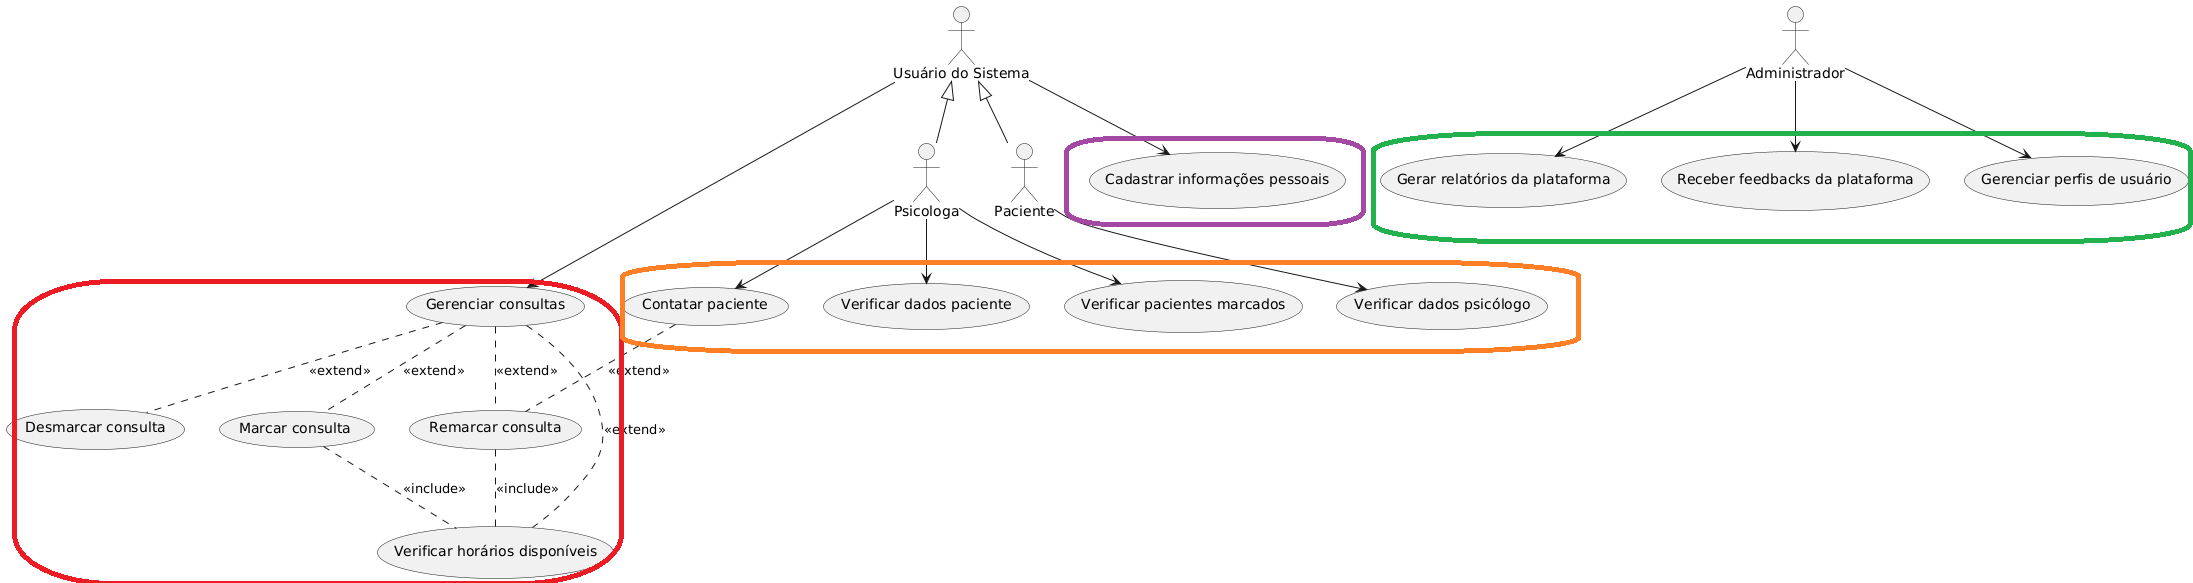
\includegraphics[width=1.0\linewidth]{casosdeuso(agrupado).png}
    \caption{Identificação de Elementos de Projeto da Arquitetura}
    \label{fig:fig1}
\end{figure}

\begin{figure}[h!]
    \centering
    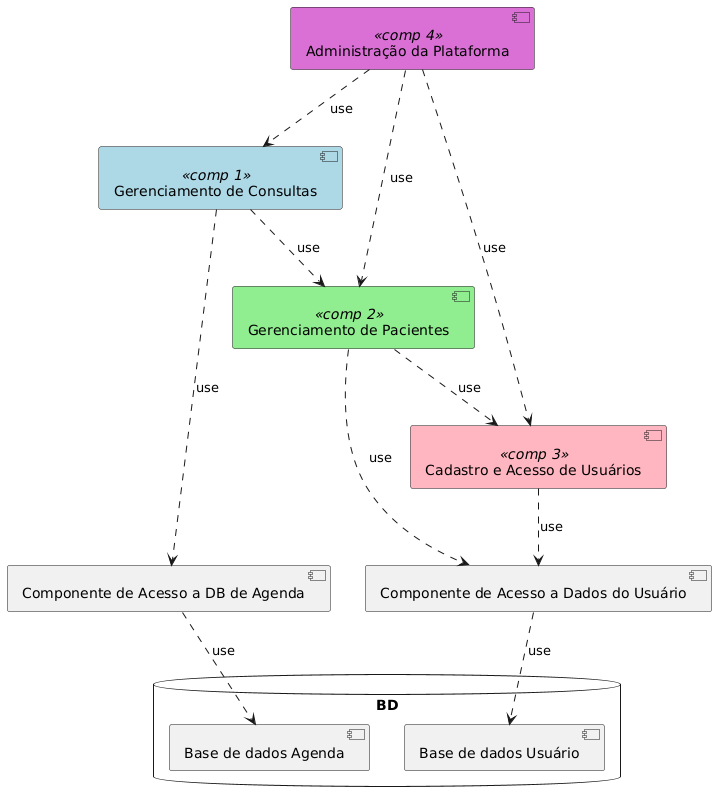
\includegraphics[width=0.5\linewidth]{diagrama_de_classes2.png}
    \caption{Diagrama de Componentes}
    \label{fig:fig2}
\end{figure}

\section{Descrição dos Componentes}
\subsection{Componente de Gerenciamento de Consultas}
\textit{Na Figura 3.1, foi representado pela união em Vermelho.} \\ 
\\
\textbf{Responsabilidades:} 
Este componente é responsável por todas as operações relacionadas à gestão das consultas, incluindo marcação, remarcação e cancelamento. Suas responsabilidades incluem:
\begin{itemize}
    \item \textbf{Marcar consulta:} Permite o agendamento de uma consulta dentre os horários disponíveis.
    \item \textbf{Remarcar consulta:} Possibilita a mudança de data ou horário de uma consulta previamente agendada, garantido que o novo horário seja escolhido de acordo com a disponibilidade do psicólogo.
    \item \textbf{Desmarcar consulta:} Facilita o cancelamento de consultas previamente agendadas, com atualização automática da agenda do psicólogo, de forma a tornar o horário vago novamente.
    \item \textbf{Verificar horários disponíveis:} Garante que o paciente possa visualizar os horários disponíveis de cada psicólogo nos momentos em que vai marcar ou remarcar uma consulta. 
\end{itemize}

Esse componente centraliza todas as interações necessárias para o gerenciamento das consultas e mantém a agenda dos psicólogos e pacientes atualizada, permitindo uma experiência de agendamento sem conflitos.


\subsection{Componente de Acesso a Informações de Pacientes e Psicólogos}
\textit{Na Figura 3.1, foi representado pela união em Laranja.} \\ 
\\
\textbf{Responsabilidades:} 
Este componente é responsável por fornecer e gerenciar as informações dos pacientes e psicólogos que utilizam a plataforma. Suas principais funções incluem:
\begin{itemize}
    \item \textbf{Verificar dados do paciente:}  Permite que os psicólogos acessem as informações básicas dos pacientes que marcaram consultas com eles, garantindo que eles estejam preparados para o atendimento.
    \item \textbf{Verificar dados do psicólogo:} Fornece aos pacientes informações sobre os psicólogos como suas especialidades.
    \item \textbf{Verificar pacientes marcados:} Ajuda os psicólogos a gerenciar a lista de pacientes que têm consultas agendadas com eles, permitindo uma melhor organização e preparo para as consultas.
    \item \textbf{Contatar paciente:} Oferece um canal direto para que o psicólogo entre em contato com o paciente, seja para enviar mensagens sobre consultas ou notificações importantes.
\end{itemize}

Esse componente facilita a troca de informações entre pacientes e psicólogos, assegurando que ambos tenham acesso aos dados necessários para o agendamento e o atendimento.

\subsection{ Componente de Cadastro e Acesso de Usuários}
\textit{Na Figura 3.1, foi representado pela união em Roxo.} \\ 
\\
\textbf{Responsabilidades:} 
Este componente gerencia o processo de criação de contas, garantindo que pacientes e psicólogos possam acessar suas funcionalidades de forma segura e personalizada. Suas principais responsabilidades incluem:

\begin{itemize}
    \item \textbf{Cadastrar informações Pessoais:} Permite que os usuários (tanto pacientes quanto psicólogos) criem uma conta na plataforma, fornecendo informações pessoais.
\end{itemize}

Esse componente é crucial para garantir a segurança e o controle de acesso à plataforma, assegurando que os dados pessoais e profissionais dos usuários sejam protegidos e que apenas usuários registrados possam utilizar os serviços oferecidos.


\subsection{ Componente de Administração da Plataforma}
\textit{Na Figura 3.1, foi representado pela união em Verde.} \\ 
\\
\textbf{Responsabilidades:} 
Este componente é destinado aos administradores do sistema e permite a supervisão e manutenção da plataforma. Ele fornece ferramentas para o gerenciamento de perfis, coleta de feedbacks e geração de relatórios para garantir o bom funcionamento e a melhoria contínua do sistema. Suas responsabilidades incluem:

\begin{itemize}
    \item \textbf{Gerenciar perfis de usuário:} Oferece aos administradores a capacidade de visualizar e gerenciar os perfis de pacientes e psicólogos, garantindo que as informações estejam corretas e atualizadas.
    \item \textbf{Receber feedbacks da plataforma:} Permite que pacientes e psicólogos enviem feedbacks sobre a plataforma, relatando problemas ou sugerindo melhorias. Os administradores podem revisar essas informações e tomar ações para melhorar a experiência do usuário.
    \item \textbf{Gerar relatórios da plataforma:} Gera relatórios sobre o uso da plataforma, como número de consultas realizadas, usuários ativos, e outras métricas relevantes, ajudando os administradores a monitorar e melhorar o sistema.
\end{itemize}

Esse componente garante que os administradores tenham controle sobre os principais aspectos do sistema, permitindo a gestão eficaz da plataforma e assegurando a qualidade do serviço oferecido.

% 4. Seção: Modelo de Classes
\chapter{Modelo de Classes}

\section{Diagrama de Classes}

\begin{figure}[h!]
    \centering
    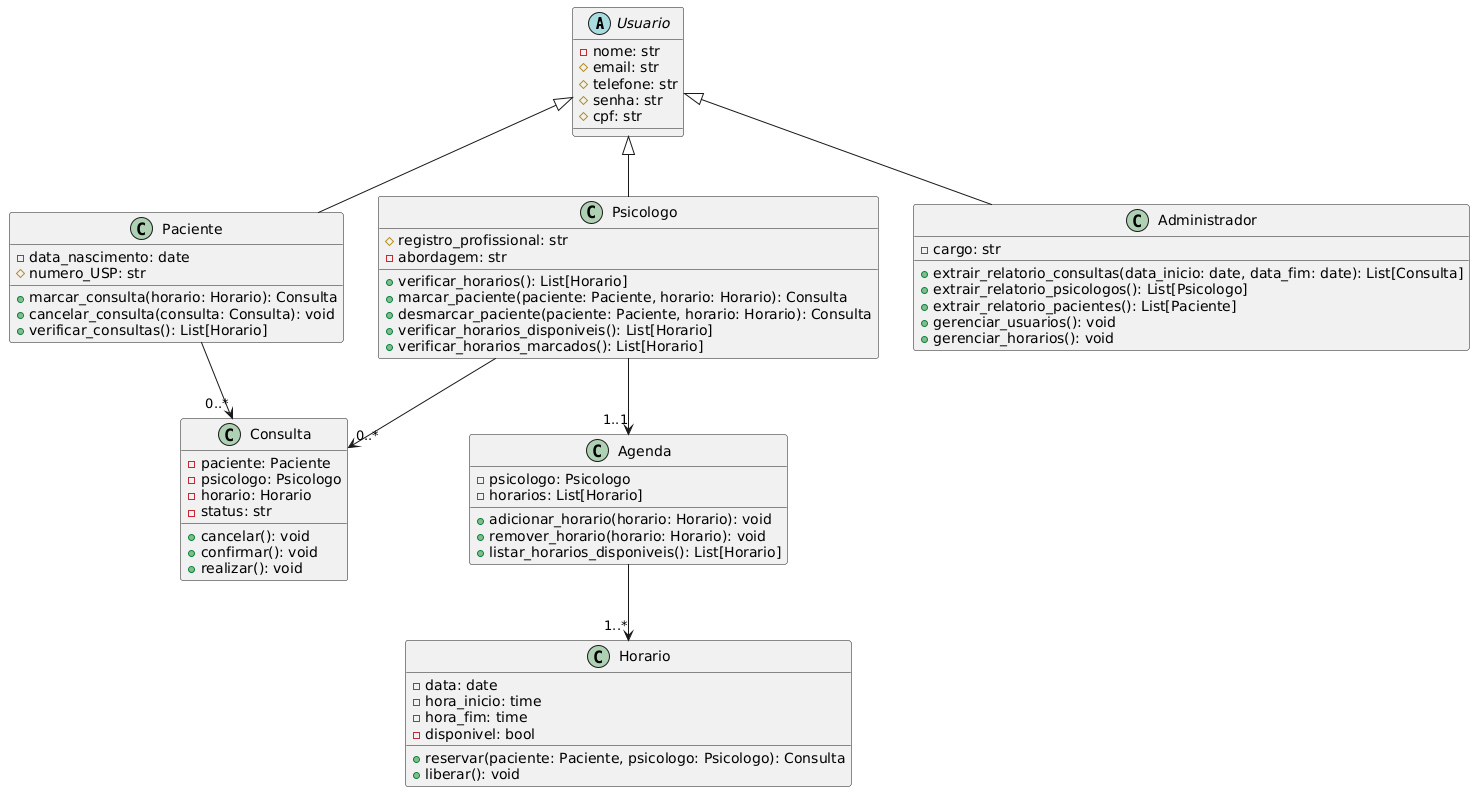
\includegraphics[width=1.0\linewidth]{diagrama_de_classes.png}
    \caption{Diagrama de Classes do Sistema}
    \label{fig:enter-label}
\end{figure}

\section{Discussão do Modelo}

\subsection{Dificuldades e Desafios}

Durante o desenvolvimento do projeto, enfrentamos diversos desafios. Inicialmente, a escolha de um tema foi um dos primeiros obstáculos. Buscávamos algo que fosse relevante para a comunidade, tivesse conexão com os conteúdos da matéria e refletisse nossa realidade. Mais adiante, ao realizar as tarefas, surgiram dificuldades na definição clara dos requisitos, especialmente devido aos diferentes tipos de usuários que o sistema precisaria atender, além de estabelecer com precisão o que deveria ser implementado.

A modelagem dos casos de uso também se revelou uma atividade complexa. Identificar corretamente as relações entre os casos, os atores envolvidos, bem como definir as pré-condições e pós-condições de cada cenário, exigiu muita atenção e ajustes. Além disso, o agrupamento desses casos para montar os componentes foi uma tarefa desafiadora, que demandou um planejamento cuidadoso.

Na fase final, um dos maiores desafios foi a definição das classes, seus atributos e a visibilidade de cada atributo. Como ainda não havíamos iniciado a implementação, pensar com clareza nesses detalhes previamente foi uma tarefa especialmente difícil, exigindo um alto nível de abstração e planejamento.

\subsection{Aprendizados Importantes}

Tivemos diversos aprendizados durante a primeira etapa do projeto. Ela nos mostrou com clareza a importância de modelar e planejar o sistema de forma correta e antecipada, de modo a facilitar as futuras etapas de implementação e tornar ajustes e correções mais simples. Desde a definição dos requisitos até a estruturação das classes, percebemos que tudo precisa ser cuidadosamente pensado com antecedência, e isso se revelou mais desafiador do que inicialmente imaginávamos.

Além disso, o projeto exigiu uma comunicação eficaz entre os membros da equipe para garantir que todas as ideias e visões sobre o projeto fossem alinhadas e esclarecidas. Esse alinhamento foi crucial para o andamento do trabalho. Outro aprendizado valioso foi o desenvolvimento de nossas habilidades de abstração e previsão de cenários, que são essenciais para a construção de um software robusto e funcional.

\end{document}
